
\section*{Ročníkový projekt 2024}

Vrámci tohoto ročníkového projektu sa budeme venovať popisu schém a konkrétnych súčastí napäťového zdroja a komunikačného rozhrania pre \href{https://github.com/ostertag/UACS}{UACS (University Access Controll System)}. Tento projekt stavia aj na poznatkoch z predošlej práce na \href{https://gitlab.com/project-deadlock}{projekte Deadlock}.

\subsection*{Napäťový zdroj}

Napäťový zdroj nám v našej implementácii slúži na zmenu vstupného napätia 12 V alebo 5 V na 3.3 V

\begin{figure}[h!]
    \centerline{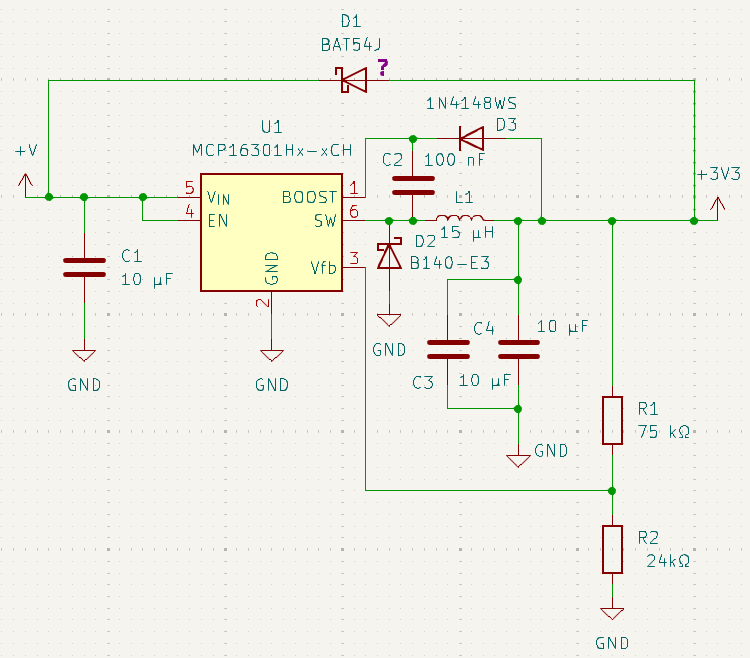
\includegraphics[width=0.9\textwidth]{schematic_power_suplly.png}}
    \caption{Schéma zapojenia napäťového zdroja}
    \label{obr:shc1}
\end{figure}


Schéma je použitá z \href{https://github.com/ostertag/UACS/blob/hardwear_kozuch/power_suply_shc_1/Data_sheet.pdf}{dátového listu} súčiastky
MCP16301Hx-xCH, konkrétne Figure 6-1 na strane 23.
\begin{figure}[h!]
    \centerline{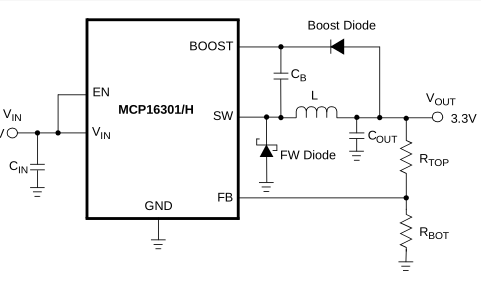
\includegraphics[width=0.9\textwidth]{sch_original.png}}
    \caption{Figure 6-1 }
    \label{obr:shc2}
\end{figure}
Niektoré externé komponenty vieme upraviť, aby sme dostali iné výsledné
napätie, prípadne iný prúd.
Naša schéma s ktorou pracujeme predpokladá vstupné napätie 12V prípadne
5V a výstupné napätie 3.3V.
Externé komponenty sú: 
\begin{itemize}

\item 
    rezistory: 
    \begin{itemize}
        \item 
        rezistory $R_1$ a $R_2$:
        \begin{itemize}
            \item 
            v dátovom liste sú to $R_{TOP}$ ($R_1$) a $R_{BOT}$ ($R_2$)
            \item 
            od ich hodnôt závisí výstupné napätie
            \item 
            v dátovom liste máme rovnicu na výpočet odporov jednotlivých rezistorov:

            \begin{equation}
                    R_{1} = R_{2} \times \left(\frac{V_{OUT}}{V_{FB}} - 1\right)
            \end{equation}
            \item
            naše $V_{OUT}$ je napätie ktoré chceme dostať na výstupe a $V_{FB}$ je napätie idúce do $V_{FB}$ pinu a musí mať hodnotu 0.8V
            \item 
            na nájdenie hodnôt rezistorov môžeme použiť script \href{https://github.com/ostertag/UACS/tree/hardwear_kozuch/power_suply_shc_1/find_rezistor}{find\_rezistor.py}
            \item 
            snažíme sa hľadať rezistory z čo najnižších sérii
            \item 
            v dátovom liste uvádzajú že $R_2$ by mal mať 10 $k\Omega$ a $R_1$ by mal mať 31.6 $k\Omega$ pre výstupné napätie 3.3V
            \item 
            my použijeme hodnoty ktoré nám našiel skript a to 75 $k\Omega$ pre $R_1$  a 24 $k\Omega$ pre $R_2$ z dôvodu že malé hodnoty odporov majú veľký stratový prúd.  
        \end{itemize}
    \end{itemize}
\item
  kondenzátory:

  \begin{itemize}
  \item
    kondenzátor $C_1$:

    \begin{itemize}
    
    \item
      v dátovom liste je to aj $C_{IN}$
    \item
      v dátovom liste je uvedené že treba použiť dva paralelne zapojené
      kondenzátory, každý o hodnote 4.7 µF
    \item
      používame 10 µF kondenzátor aby sme znížili množstvo komponentov a
      náročnosť zapojenia
    \end{itemize}
  \item
    kondenzátory $C_3$ a $C_4$:

    \begin{itemize}
    
    \item
      v dátovom liste je to aj $C_{OUT}$
    \item
      ich hodnota zavisí od výsledného napätia
    \item
      pre naše výstupné napätie používame dva kondenzátory každý o
      hodnote 10 µF, ktoré budú paralelne zapojené
    \end{itemize}
  \item
    pri hodnotách kondenzátorov sa riadime tabuľkou 5-2 na strane 18:

    \begin{longtable}[]{@{}lll@{}}
    \toprule\noalign{}
    Parameter & Min & Max \\
    \midrule\noalign{}
    \endhead
    \bottomrule\noalign{}
    \endlastfoot
    $C_{IN}$ & 2.2 µF & None \\
    $C_{OUT}$ & 20 µF & None \\
    \end{longtable}
  \item
    zároveň minimálna napätie kondenzátorov musí byť napätie ktoré nimi
    maximálne môže prechádzať plus nejaká rezerva

    \begin{itemize}
    
    \item
      Ako rezervu zvyčajne používame hodnotu maximálneho napätia, ktoré môže kondenzátorom prechádzať, takže napätie kondenzátorov bude dvojnásobkom maximálneho napätia, ktoré nimi môže prechádzať.
    \end{itemize}
  \end{itemize}
\item
  cievka:

  \begin{itemize}
  \item
    používame 15 µH cievku
  \item
    podľa výstupného napätia upravujeme jej hodnotu podľa tejto rovnice:

    \[K = V_{OUT}/L\]
  \item
    kde K by malo mať hodnotu 0.22 V/µH a $V_{OUT}$ je naše výstupné napätie
    (3.3V)
  \item
    pre iné napätia sa môžeme riadiť tabuľkou 5-1 na strane 17

    \begin{longtable}[]{@{}lll@{}}
    \toprule\noalign{}
    $V_{OUT}$ & K & $L_{STANDART}$ \\
    \midrule\noalign{}
    \endhead
    \bottomrule\noalign{}
    \endlastfoot
    2.0V & 0.20 & 10 µH \\
    3.3V & 0.22 & 15 µH \\
    5.0V & 0.23 & 22 µH \\
    12V & 0.21 & 56 µH \\
    15V & 0.22 & 68 µH \\
    \end{longtable}
  \end{itemize}
\item
  ostatné externé komponenty aj ich charakteristiky vieme nájsť v
  dátovom liste na stranách 19 až 20
  \item 
  v pôvodnom návrhu z projektu Deadlock, bola v schéme umiestnená dióda BAT54, nakoľko si nie sme istý dôvodom umiestnenia tejto diódy, je pri nej v schéme otáznik 
\end{itemize}

\subsection*{Komunikačné rozhranie}

\begin{figure}[!h]
    \centerline{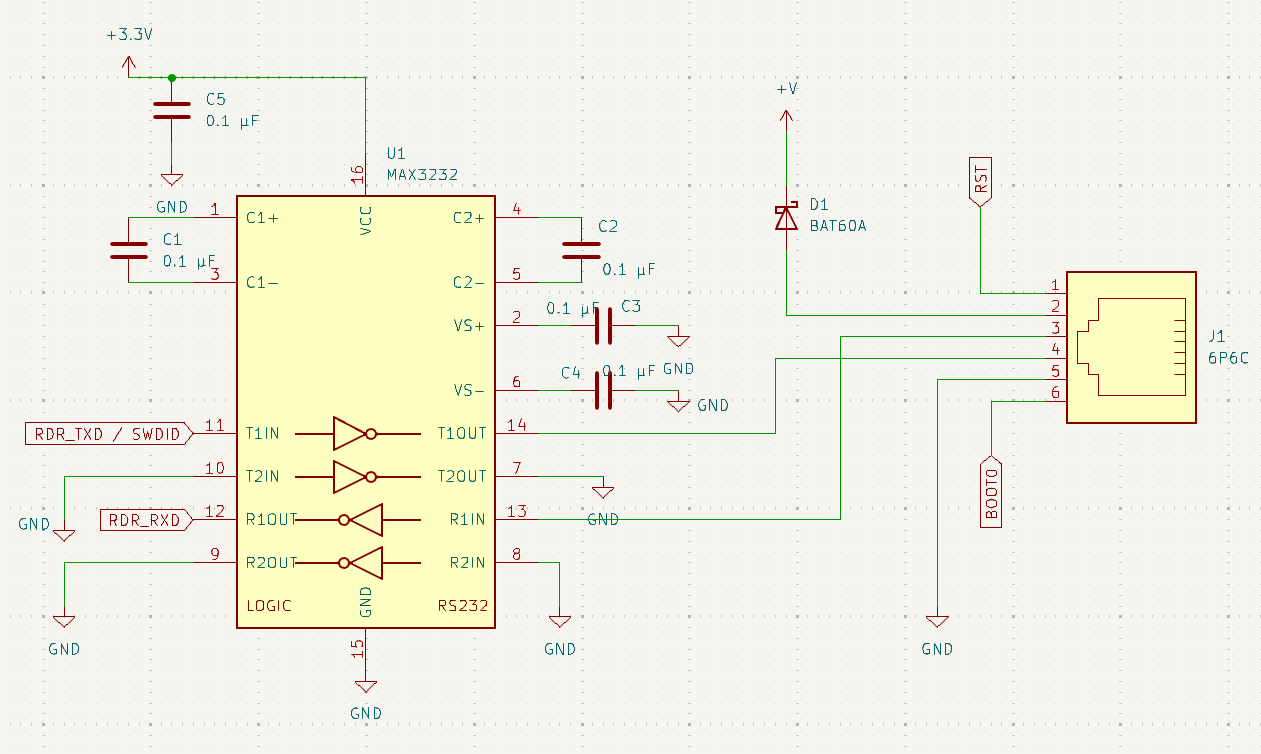
\includegraphics[width=0.9\textwidth]{rs-232_schematic.png}}
    \caption{Schéma zapojenia komunikačného rozhrania}
    \label{obr:shc1}
\end{figure}

Komunikačné rozhranie sa skladá z dvoch komponentov:
\begin{itemize}
\item 
  RJ12 konektor 6p6c:
  \begin{itemize}
   \item 
  slúži na komunikáciu s externou súčiastkou, ktorá môže byť pripojená prostredníctvom kábla s RJ12 konektormi
  \item 
  slúži zároveň aj ako napájanie celého zariadenia napätím medzi 4V až 15V
  \item 
  funkcie jednotlivých pinov konektora sú v tejto tabuľke:

\begin{longtable}[]{@{}ll@{}}
  \toprule\noalign{}
  Pin & Funkcia\\
  \midrule\noalign{}
  \endhead
  \bottomrule\noalign{}
  \endlastfoot
  1 & RST \\  
  2 & Napájanie\\
  3 & Transmit \\
  4 & Receive \\
  5 & Zem \\
  6 & BOOT0\\
  \end{longtable}

\item
  pin1 budeme používať pre RST signál
\item
  pin2 budeme používať pre napájanie
\item
  pin3 budeme používať na prijímanie signálu do nášho MCU, zatiaľ čo na druhej strane kábla bude použitý na vysielanie
\item
  pin4 budeme používať na odosielanie signálu z nášho MCU, zatiaľ čo na druhej strane kábla bude použitý na prijímanie
\item
  pin5 pripojíme na zem
\item
  pin6 budeme používať pre BOOT0 signál
  \end{itemize}
  \item 
  MAX3232

  \begin{itemize}
  \item
    schému zapojenia používame z \href{https://github.com/ostertag/UACS/blob/hardwear_kozuch/rs-232_interface/Data_sheet.pdf}{dátového listu}
    zo strany 12
    \begin{figure}[!h]
        \centering
        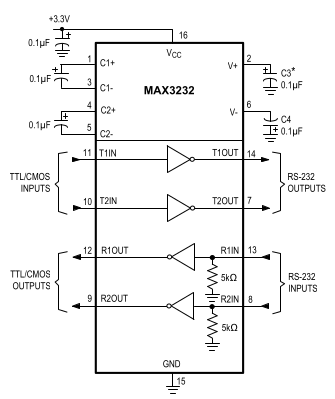
\includegraphics[width=0.5\linewidth]{org_sch.png}
        \caption{Schéma z dátového listu na strane 12}
        \label{fig:enter-label}
    \end{figure}
  \item
    vrámci RS-232 štandardu sú napätia pre logickú jednotku a nulu
    definované takto:
  \end{itemize}

  \begin{longtable}[]{@{}cc@{}}
  \toprule\noalign{}
  Logická hodnota & Napätie \\
  \midrule\noalign{}
  \endhead
  \bottomrule\noalign{}
  \endlastfoot
  0 & +3 až +15 V \\
  1 & -15 až -3 V \\
  \end{longtable}

  \begin{itemize}
  
  \item
    pri prijímaní signálu MAX 3232 konvertuje vstupné napätie na napätie
    pre logickú nulu (0V až 0.8V) alebo jednotku(2V až 3.3V)
  \item
    pri odosielaní signálu konvertuje napätie logickej nuly alebo
    jednotky na napätie +5V až +5.4V alebo -5V až -5.4V 
  \item
    pre podrobnejšie informácie treba pozrieť tabuľku na strane na strane 2 až 3 (Electrical Characteristics)
  \item
    funkcie jednotlivých pinov sú v tejto tabuľke, nájdeme ju na strane
    6 v dátovom liste:
  \end{itemize}

  \begin{longtable}[]{@{}lll@{}}
  \toprule\noalign{}
  Pin & Meno & Funkcia \\
  \midrule\noalign{}
  \endhead
  \bottomrule\noalign{}
  \endlastfoot
  1 & C1+ & Positive Terminal of Voltage-Doubler Charge-Pump
  Capacitor \\
  2 & V+ & +5.5V Generated by the Charge Pump \\
  3 & C1- & Negative Terminal of Voltage-Doubler Charge-Pump
  Capacitor \\
  4 & C2+ & Positive Terminal of Inverting Charge-Pump Capacitor \\
  5 & C2- & Negative Terminal of Inverting Charge-Pump Capacitor \\
  6 & V- & -5.5V Generated by the Charge Pump \\
  7,14 & T\_OUT & RS-232 Transmitter Outputs \\
  8,13 & R\_IN & RS-232 Receiver Inputs \\
  9,12 & R\_OUT & TTL/CMOS Receiver Outputs \\
  10, 11 & T\_IN & TTL/CMOS Transmitter Inputs \\
  15 & GND & Ground \\
  16 & $V_{CC}$ & +3.0V to +5.5V Supply Voltage \\
  \end{longtable}

  \begin{itemize}
  \item
    piny 1 až 6 sú súčasťou takzvanej ``Charge pump''

    \begin{itemize}
    \item
      slúži na zvýšenie napätia, aj keď vstupné napätie je nižšie
    \item
      v našom prípade zvyšuje zo vstupného napätia 3.3V na 5.5V alebo
      -5.5V
    \end{itemize}
  \item
    piny 7 a 14 posielajú výstupný signál o hodnote medzi -3V až -15 V
    alebo 3V až 15V
  \item
    piny 8 a 13 prijímajú vstupný signál o hodnote medzi -3V až -15 V
    alebo 3V až 15V
  \item
    piny 9 a 12 posielajú výstupný signál ktorý je buď logická nula
    alebo jednotka
  \item
    piny 10 a 11 prijímajú vstupný signál ktorý je buď logická nula
    alebo jednotka
  \item
    pin 15 je uzemnený
  \item
    pin 16 je určený pre napájanie súčiastky
  \item
    v našej implementácii:

    \begin{itemize}
    \item
      pre posielanie signálov používame dvojicu pinov 11 a 14
    \item
      pre prijímanie signálov používame dvojicu pinov 12 a 13
    \end{itemize}
  \item
    jediné externé súčiastky sú kondenzátory, ich minimálne hodnoty pre
    dané napätie sú v tabuľke 2 na strane 9:

    \begin{longtable}[]{@{}lll@{}}
    \toprule\noalign{}
    $V_{CC}$ (V) & C1 (µF) & C2, C3, C4 (µF) \\
    \midrule\noalign{}
    \endhead
    \bottomrule\noalign{}
    \endlastfoot
    3.0 to 3.6 & 0.1 & 0.1 \\
    4.5 to 5.5 & 0.047 & 0.33 \\
    3.0 to 5.5 & 0.1 & 0.47 \\
    \end{longtable}
  \item
    vieme použiť vyššie hodnoty kondenzátorov, zvlášť ak kondenzátory
    ktoré používame menia svoju hodnotu s rastúcou teplotou
  \item
    ak chceme zvýšiť hodnotu kondenzátora C1 musíme zvýšiť aj hodnoty
    ostatných kondenzátorov
  \item
    pri zvyšovaní hodnôt kondenzátorov C2 , C3 a C4 nemusíme zvyšovať
    hodnotu kondenzátora C1
  \item
    kondenzátor C5 používame v prípade ak je naša implementácia citlivá
    na ``hluk'' zdroja
  \item
    kondenzátor C5 bude mať rovnakú hodnotu ako kondenzátor C1
  \item
    pre viacej detailov ohľadom kondenzátorov pozri strany 8, 9
    (Capacitor Selection, Power-Supply Decoupling) v dátovom liste
  \item
    piny ktoré nebudú na nič pripojené, pripojíme na zem, prípadne na
    $V_{cc}$ (pozri stranu 7 - RS-232 Transmitters v dátovom liste)
  \end{itemize}
\end{itemize}

